\documentclass[11pt,a4paper]{article}
\usepackage[margin=2.2cm]{geometry}
\usepackage[T1]{fontenc}
\usepackage{lmodern}
\usepackage{microtype}
\usepackage{amsmath}
\usepackage{xcolor}
\usepackage{booktabs}
\usepackage{tabularx}
\usepackage{xltabular}
\emergencystretch=3em
\usepackage{enumitem}
\usepackage{listings}
\usepackage{tikz}
\usetikzlibrary{arrows.meta,positioning,automata}
\usepackage[colorlinks=true,linkcolor=blue!50!black,urlcolor=blue!50!black]{hyperref}

\definecolor{codebg}{gray}{0.96}
\lstset{basicstyle=\ttfamily\small,backgroundcolor=\color{codebg},frame=single,rulecolor=\color{gray!40},
  columns=fullflexible,keepspaces=true,breaklines=true,showstringspaces=false}
\newcommand{\f}[1]{\texttt{#1}}
\lstdefinelanguage{Rust}{morekeywords={fn,let,mut,pub,struct,enum,impl,match,if,else,for,in,return,Some,None,true,false,self,Self,use,const,as,while,loop},
  sensitive=true,morecomment=[l]{//},morestring=[b]"}
\lstset{keywordstyle=\color{blue!60!black}\bfseries}
\setlist{nosep,leftmargin=1.4em}
\setlength{\parindent}{0pt}
\setlength{\parskip}{5pt}

\title{The League --- how our bot trains itself}
\author{Patient Wolves, Battlecode 2026a, branch \f{league}}
\date{October 2026}

\begin{document}
\maketitle

\section*{Quick start}
\textbf{0. Set up a PC once} (a teammate's desktop, your laptop: any Windows PC). The person needs
push access to the GitHub repo, because results are shared by pushing to \f{league}:
\begin{lstlisting}
git clone -b league https://github.com/Ahmed-Abdul-Rahim/battlecode-2026a.git
cd battlecode-2026a
powershell -ExecutionPolicy Bypass -File scripts\setup.ps1
\end{lstlisting}
Then open PowerShell in the repo folder and activate the environment once per window:
\begin{lstlisting}
.\.venv\Scripts\Activate.ps1
\end{lstlisting}

\textbf{1. Start the work} (each runs in the background until you stop it):
\begin{lstlisting}
scripts\train.ps1 start                          # any PC: tune the numbers per map
scripts\train.ps1 experiments                    # any PC: test the queued ideas
scripts\train.ps1 ml                             # optional: data games + network training
scripts\train.ps1 start --lead --auto-submit     # the ONE lead PC only: ladder + uploads
\end{lstlisting}
\textbf{Which to run:} on a teammate's PC or a laptop, \f{start} and \f{experiments}. Two processes
per PC is enough: each already uses every core but two, so a third only shares the same CPU. Only
one PC in the team may use \f{-{}-lead}; \f{-{}-auto-submit} also needs \f{cambc login}. The upload
rules are in \S\ref{sec:release}.

\textbf{Stop} before you shut down or carry a laptop away (unfinished work returns to the shared
queue):
\begin{lstlisting}
scripts\train.ps1 stop
scripts\train.ps1 experiments stop
scripts\train.ps1 ml stop
\end{lstlisting}
\textbf{Laptops:} keep them plugged in and set ``when I close the lid'' to \emph{Do nothing}
(Control Panel, Power Options), or a sleeping laptop holds its claimed experiment for up to 6 hours.
Each PC is known by its computer name; if two share one, set \f{\$env:LEAGUE\_HOST = "laptop"} before
starting. \textbf{After a change to \f{harness/}} (the Python), restart: \f{stop}, then \f{start} and
\f{experiments} again. Bot code and new queue items reach every PC by themselves.

\textbf{More PCs = faster, not linearly:} an 8-core laptop adds about half of what a 16-core desktop
does, and each experiment still runs whole on one PC; the queue just drains faster.

\textbf{Try an idea you found} (a gap in a replay, a new rule). Queue it; every PC's autopilot picks
it up, and the result lands in the registry (Appendix~\ref{sec:registry}):
\begin{lstlisting}
# an existing switch: just a value
scripts\train.ps1 experiments add --title "Hunt carriers late" --area teamwork --knobs HUNT_MODE=2

# new code: write it behind a new knob2 switch on a branch, push the branch, then
git switch -c feat/my-idea      (code, cargo test, then: git push -u origin feat/my-idea)
scripts\train.ps1 experiments add --title "My idea" --area combat --ref origin/feat/my-idea --knobs MY_IDEA=1

scripts\train.ps1 experiments add ... --first   # test it before everything else in the queue
scripts\train.ps1 experiments list              # queue and results (short)
scripts\train.ps1 exp-status                    # readable report: running, merged,
                                                #   rejected (and why), up next
\end{lstlisting}
The branch is merged onto the live code before every test, so keep it small; if it conflicts, the
command says ``needs rebase'' (run \f{git merge origin/league} on the branch, push, add again).

\textbf{Experiments run by themselves but do not merge by themselves.} A winner shows
\f{passed} in \f{experiments list}. To ship it: set its switch's default in
\f{crates/bc-core/src/memory.rs} (and merge its branch if it has one), run \f{python -m bctools.sync},
\f{cargo test}, commit and push to \f{league}. Every PC picks it up; the next upload carries it.

\textbf{2. See how the latest model is doing:}
\begin{lstlisting}
scripts\train.ps1 status        # version, win rate per top team, losses
scripts\train.ps1 logs          # live log (Ctrl+C to leave)
scripts\train.ps1 bench         # new test vs every mimic, every map
scripts\train.ps1 review        # full report: league\review\<date>.md
\end{lstlisting}

\textbf{3. Watch it play} (opens the official viewer in your browser):
\begin{lstlisting}
scripts\train.ps1 replay                    # our worst team + map
scripts\train.ps1 replay nyx lanes          # vs Nyx's mimic on lanes
scripts\train.ps1 replay nyx lanes --evolved   # vs the harder Nyx
\end{lstlisting}
It plays two games (one from each side) and prints win/loss and gems. The viewer opens the first game, and the
command for the second is printed. Stop the viewer with Ctrl+C. Real ladder games:
\f{cambc matches download <matchId> -o x.repl26a}, then \f{cambc view x.repl26a}.

\section{The idea in five sentences}
\begin{enumerate}
\item We copy the 10 best teams on the ladder into practice bots, called \textbf{mimics}.
\item Our bot plays thousands of games against these mimics on every map.
\item After each batch of games we try small changes to our bot's numbers, and keep the changes that win more.
\item When we lose on the real ladder, the bot trains on that map first, and a better version can be uploaded.
\item Anything the training cannot fix is written in a report for a human to look at.
\end{enumerate}
Every teammate's PC runs the same program (\f{harness/league.py}). They share the results through git.

\section{One training round}
\begin{center}
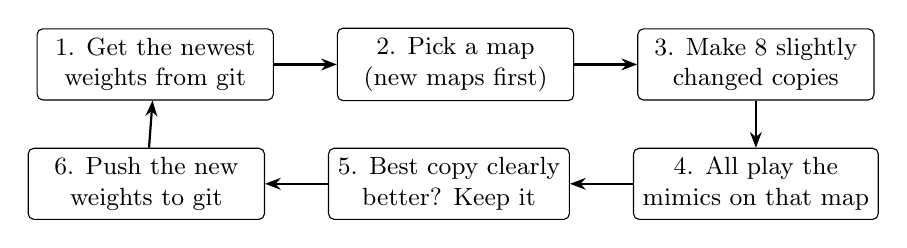
\begin{tikzpicture}[node distance=6mm and 8mm,
  box/.style={draw,rounded corners=2pt,align=center,font=\small,minimum width=30mm,minimum height=9mm},
  arr/.style={-{Stealth[length=2mm]},thick}]
  \node[box] (a) {1. Get the newest\\weights from git};
  \node[box,right=of a] (b) {2. Pick a map\\(new maps first)};
  \node[box,right=of b] (c) {3. Make 8 slightly\\changed copies};
  \node[box,below=of c] (d) {4. All play the\\mimics on that map};
  \node[box,left=of d] (e) {5. Best copy clearly\\better? Keep it};
  \node[box,left=of e] (f) {6. Push the new\\weights to git};
  \draw[arr] (a)--(b); \draw[arr] (b)--(c); \draw[arr] (c)--(d); \draw[arr] (d)--(e); \draw[arr] (e)--(f);
  \draw[arr] (f)--(a);
\end{tikzpicture}
\end{center}
A round takes about 4 minutes. Every third round, we train one of the \emph{mimics} instead of our bot
(see \S\ref{sec:opp}).

\textbf{Which map gets trained.} In this order:
\begin{enumerate}
\item \textbf{Maps that were never trained} (new maps, or old ones still on default numbers). Each gets 4 rounds
  first, and maps we lost on the ladder go first.
\item \textbf{The oldest ladder loss of the version that is live now}, unless its map already had 6 rounds
  since that loss. After that it goes to the human review.
\item \textbf{Where we keep losing:} a weighted pick by ``map pressure'', meaning recent ladder losses on
  that map (a loss counts less every day, and double if the live version lost it), times how badly we
  do on that map locally. Every map keeps a small share, so none is forgotten.
\end{enumerate}
\textbf{When a new version is uploaded,} the open losses are marked \emph{superseded}: they leave the
queue, because they were losses of the old version, but they stay in the review and still count in map
pressure. So training never runs out of work and never replays an endless queue.
Every map in the platform's pool always has an entry: a new map starts with the default numbers
until training improves them. \f{train status} checks that the counts agree
(\emph{fingerprint 21/21, geometry 21/21, in pack 21/21, trained N/21}). It also lists each untrained
map with its rounds so far, e.g. \emph{hooks 2/4}. A map without a fingerprint is never trained,
because the bot couldn't load its numbers, and \f{status} reports it as OUT OF SYNC.

\section{What the bot learns}\label{sec:learn}
\subsection*{Code vs numbers}
Our bot is hand-written Rust code. The code decides \emph{how} to do things: find a path, attack,
buy an item, deliver gems. Many of its decisions compare options with a formula, and those formulas
contain numbers. Training never touches the code. It only changes these \textbf{169 numbers}
(67 of them belong to features that are still switched off, so training leaves them alone).

Each map has its own set of 169 numbers. On a small map with camps close together, walking distance
matters less than on a big map. On a map where fights happen early, retreating sooner may be better.
A map we never trained on uses the default numbers in \f{bots/main/src/learned.rs}.

The numbers come in five groups.

\subsection*{1. W --- 18 dials on our own settings}
While writing the bot we picked many settings by hand, such as ``retreat at 35\% HP''. Each W number
\emph{multiplies} one such setting. 1.0 means ``as we wrote it'', 1.2 means 20\% more, and 0.8 means
20\% less. For example, if the written retreat point is 35\% HP, a \f{retreat\_hp} of 1.2 makes the
bot retreat at 42\%. Allowed range: 0.2 to 5.

\begin{tabularx}{\linewidth}{@{}lX@{}}
\toprule
Dial & What turning it up does\\
\midrule
\f{gem}, \f{gold} & Camps with more gems / gold look more attractive.\\
\f{dist}, \f{opening\_dist} & Walking distance counts more, so near camps win (\f{opening\_} only at game start).\\
\f{clear} & Time needed to kill a camp counts more, so quick camps win.\\
\f{strength\_discount} & Strong (dangerous) camps look less attractive.\\
\f{reward}, \f{shared\_small} & Bonus for camps that drop items; how much a small camp shared with allies is worth.\\
\f{hysteresis} & Stick with the current target instead of switching back and forth.\\
\f{en\_detour}, \f{en\_clear} & Allow longer detours and harder camps when clearing ``on the way''.\\
\f{fight\_margin} & Need a bigger advantage before starting a fight (more careful).\\
\f{retreat\_hp} & Retreat earlier (at higher HP).\\
\f{aggression} & Chase and attack enemies more.\\
\f{recall\_gold} & Carry more gold before going home to shop.\\
\f{tribute\_min}, \f{tribute\_max} & Carry more gems before walking to the altar to deliver them.\\
\f{assist\_hp} & Need more HP before running to help a teammate.\\
\bottomrule
\end{tabularx}

\subsection*{2. TARGET --- 10 weights for ``which camp next?''}
Every time a champion picks its next camp, it gives each camp a score from the dials above. The TARGET
weights then adjust that score with 10 facts about the camp:
\begin{center}
gems in it \textbullet{} gold in it \textbullet{} distance \textbullet{} time to clear \textbullet{} time until it respawns
\textbullet{} how many others are going for it \textbullet{} damage we would take \textbullet{} how full our bag is
\textbullet{} our emblem count \textbullet{} the game round
\end{center}
Each weight is a number from $-3$ to $+3$, and 0 means ``ignore this fact''. A positive weight on
\emph{round} makes far camps more attractive late in the game. A negative weight on \emph{damage}
avoids camps that hurt. The camp's score is multiplied by $e^{\,\text{sum of weight}\times\text{fact}}$.

\subsection*{3. FIGHT --- 9 weights for ``is this fight good?''}
Before fighting, the bot estimates its advantage. The FIGHT weights adjust that estimate with:
our HP, enemy HP, allies nearby, enemies nearby, whether we are ranged, whether they are ranged, how
full our bag is (a full bag means more to lose), and how far we are from our spawn, plus a constant.
Range $-3$ to $+3$, and 0 = off. A negative weight on \emph{bag} makes a champion carrying many gems avoid fights.

\subsection*{4. U --- 60 weights for ``what do I do right now?''}
Every turn, a small decision maker scores 6 possible actions:
\begin{center}
keep going \textbullet{} step back \textbullet{} support an ally \textbullet{} fight \textbullet{} walk home \textbullet{} recall (teleport home)
\end{center}
using 10 facts: a constant, our HP, damage per turn from camps, damage per turn from enemies, enemies
nearby, allies nearby, an ally in trouble, bag size, distance to spawn, and enemy ranged. Each action
has one weight per fact, so $6 \times 10 = 60$ numbers. The highest score wins. All zeros means ``do
what the hand-written rule says''. Range $-4$ to $+4$.

\subsection*{5. X --- 4 extras, and HOT}
\f{tavi\_respec} ($>0.5$ = Tavi re-buys its stats mid-game). \f{arbiter\_fuel\_floor}: the U decision
maker only runs when at least this much CPU fuel (25k--60k) is left in the turn, so we never freeze.
Two slots are unused. \textbf{HOT} (1 number) avoids places we died before; it is fixed at 0
because it made us worse.

\subsection*{Not learned}
These are fixed code or fixed per-map plans, and only a human can change them:
\begin{itemize}
\item pathfinding, and how attacks and spells are aimed;
\item the draft (which champions we pick);
\item emblem build order, and the shopping list;
\item which map features the bot can ``see''. If an important fact is missing from the lists above,
  no amount of training can use it. That is the ``model can't express it'' case in \S6.
\end{itemize}
See all 102 names and their current defaults: \f{python harness\textbackslash params.py -{}-list}.

\subsection*{How training changes the numbers}
One round works on one map:
\begin{enumerate}
\item Take the current best numbers for that map.
\item Make 8 copies, each nudged by a small random amount. They come in 4 mirrored pairs: one copy
  goes $+$ and its partner goes $-$, which makes the comparison fairer.
\item Every copy and the current best play the same opponents (4 mimics + 1 anchor bot) on that map,
  from both sides. That is about 90 games, run in parallel.
\item If the best copy clearly wins (see below), it becomes the new best for that map.
\item The nudge size adapts: after a success it grows by 15\% (explore further), after a failure it
  shrinks by 15\% (fine-tune).
\end{enumerate}

\subsection*{How a copy is judged}
Each bot gets a score over its games on that map:
\[ \text{score} = \text{win rate} + 0.25 \times \text{gem lead} - 0.01 \times \text{average deaths} \]
\emph{Gem lead} is $(\text{our gems} - \text{their gems}) / (\text{our gems} + \text{their gems})$, from $-1$ to $+1$. So a close
loss still scores better than a crushing loss, and dying a lot costs a little.

\textbf{Example.} The current bot wins 6 of 10 games (0.6), has an average gem lead of $+0.1$, and dies 5 times a game:
$0.6 + 0.025 - 0.05 = 0.575$. A copy that wins 7 of 10 with lead $+0.2$ and 4 deaths scores
$0.7 + 0.05 - 0.04 = 0.71$. That is 0.135 better, so it passes the first test.

A copy replaces the current best only if \textbf{all four} hold:
\begin{enumerate}
\item[(a)] its score is at least \textbf{0.04} higher on the same games (small differences are luck);
\item[(b)] it beats the current best \textbf{head-to-head} on that map (at least 50\%);
\item[(c)] it also scores at least as well against \textbf{3 other opponents} that it wasn't trained against
  (so it didn't just learn one opponent's habits);
\item[(d)] it runs out of CPU fuel no more than twice as often (a frozen champion loses games).
\end{enumerate}
Then the new numbers are saved, a full test against every mimic on every map is run, and the result
is pushed so all PCs use it. Games are deterministic: the same bots on the same map always play the
same game. Any difference between two copies therefore comes from their numbers, not from luck in the
game itself.

\section{Who we train against}\label{sec:opp}
\begin{tabularx}{\linewidth}{@{}>{\raggedright\arraybackslash}p{3.6cm}X@{}}
\toprule
\textbf{Faithful mimic} (\f{mimic-nyx}) & A copy of a real team. From their recent ladder games we copy their
  champion picks, emblem builds, first camps on each map, and how often they deliver gems and shop. Their
  fighting can't be copied (the game data doesn't show it), so a mimic fights like our own bot.
  Never changed by training, so ``our win rate vs Nyx'' stays an honest number.\\
\textbf{Evolved mimic} (\f{mimx-nyx}) & The same copy, but its numbers are trained to \emph{beat us}.
  Its picks, builds, first camps and delivery habits stay locked to the real team. If the real teams stop
  updating their bots, these keep getting harder, so our training doesn't stall. If the real team changes
  its bot, its evolved mimic starts over.\\
\textbf{Anchor bots} (\f{claude-*}, \f{exploit-*}, \f{baseline}) & Hand-written bots that attack known
  weak spots (for example killing our carrier near the altar). They stop old bugs coming back.\\
\bottomrule
\end{tabularx}
We pick opponents that beat us more often than ones we already beat.

\section{When a new version goes on the ladder}\label{sec:release}
Only one PC, the \textbf{lead}, talks to the platform. If it runs with \f{-{}-auto-submit}, it uploads the
newest trained version when \textbf{all} of these are true:
\begin{itemize}
\item the trained version is newer than the one on the ladder;
\item at least 3 hours have passed since the last upload;
\item we lost a ladder game since then, \textbf{or} the new version wins at least 5\% more against the mimics.
\end{itemize}
If the new version then does more than 10\% worse on the ladder (after 10 ranked games each), the
previous version is put back.

The 3 hours count from the last upload's time in \f{league/ledger.json}, not from when the daemon
started. The daemon checks at the start and the end of every round, so after a restart a due upload goes
out within seconds. \f{train status} shows it on the \emph{next upload} line. While the daemon runs, it
also stops Windows from going to sleep on its own; you can still put the PC to sleep yourself.

\section{What our bot can and can't do}\label{sec:can}
Status on 21 October 2026 (engine 1.0.0). ``Tested'' means we played old against new on the same games
against our copies of the top teams; ``no gain'' means it didn't win more, so it is switched off.

\subsection*{It can}
\begin{itemize}
\item \textbf{Farm camps.} It picks the next camp by gems, gold, distance and how long the camp takes to
  kill, with numbers trained for each map. It captures the reward and avoids camps an ally already claimed.
\item \textbf{Deliver gems.} It walks to an altar once its bag is big enough (bigger when the altar is far,
  smaller when it is hurt or near the end). Next to an altar it delivers from 5 gems.
\item \textbf{Shop and recall.} It goes home to buy items when it has gold, and recalls only when nothing
  can reach it during the recall.
\item \textbf{Decide fights.} It compares how fast it kills the enemy with how fast the enemy kills it
  (allies nearby included). It only switches between fighting and fleeing after two turns that agree,
  so it doesn't flip-flop.
\item \textbf{Remember fights.} It keeps a short record of recent fights and of each enemy champion type.
  After three lost exchanges, or a bad record against that type, it stops taking those fights.
\item \textbf{Finish hurt enemies.} When a teammate reports an enemy champion at half health or less
  within 4 tiles, it goes to kill it. This is PvP only.
\item \textbf{Help teammates on its way.} When a teammate calls for help and the fight is at most 4 tiles
  off its route, it joins.
\item \textbf{Stop enemy deliveries.} It stuns or attacks an enemy channelling a delivery nearby, which
  cancels it.
\item \textbf{Know the current game.} All 13 champions including Heart of Ruin, the Golem camp, and live
  champion stats read from the engine, so balance patches flow through.
\item \textbf{Share 8 bytes with its team:} which of the 10 best camps each ally is going for, the last
  enemy seen (where, how hurt, whether it is delivering), a help flag, and team-wide aggression and
  bag-size settings.
\end{itemize}

\subsection*{It can't (yet)}
\begin{itemize}
\item \textbf{Check whether it can survive a camp.} By default it doesn't, so a lone champion can walk into
  a Golem. \emph{Being tested:} a survival check, and an early-game ramp (easy camps first).
\item \textbf{See monster damage.} It treats a half-killed camp group as full health. \emph{Next test:}
  use the live health of the camps it can see.
\item \textbf{Help with monsters.} It doesn't join an ally fighting a camp next to it. \emph{Next test:} join
  within 4 tiles.
\item \textbf{Deliver on the way.} It walks past altars on its route unless it is right next to one.
  \emph{Next test:} deliver if an altar is at most 3 tiles off the route.
\item \textbf{Use bag sizes for the new economy.} They were tuned when camps paid 3--5$\times$ more gems.
  \emph{Being tested:} smaller bags.
\item \textbf{Play skill combos.} Its stun is not timed with its burst. \emph{Tested:} a ``stun first, then
  burst'' order; no gain.
\item \textbf{Dodge or kite.} It only keeps distance when it is ranged and the enemy is melee; it doesn't
  step out of spells. Melee champions don't dash in (tested; no gain).
\item \textbf{See far.} It sees only its own vision plus the one shared sighting, and forgets an enemy
  after 12 rounds.
\item \textbf{Play Heart of Ruin itself.} It knows how dangerous an enemy Heart of Ruin is at low health,
  but its draft doesn't pick it and it has no special play for it.
\end{itemize}

\subsection*{Tried and switched off (measured worse or no better)}
\begin{tabularx}{\linewidth}{@{}lX@{}}
\toprule
Idea & What happened\\
\midrule
Full combat state machine & 40\% fewer deaths, but farmed far less: win rate 0.52 $\to$ 0.43.\\
Help calls with intent (fight / escape / finish / abort) & Win rate fell; removed from the 8 bytes.\\
Travelling to answer any help call & Abandoned camps; cost more than it saved.\\
Stepping back instead of walking home & More deaths and fewer gems.\\
Stun-then-burst combo order & Slightly fewer gems; no gain.\\
Prism/Vesper ``play to the passive'' roles & Win rate 0.58 $\to$ 0.48.\\
\bottomrule
\end{tabularx}

\section{What humans do}
Every few hours the lead writes \f{league/review/<date>.md}. Read it, and write your thoughts in its
\emph{Reviewer notes} section. The program keeps that section.

\textbf{The ``gap'' column} compares our win rate against a team's mimic with our real win rate against
that team. A big gap means the mimic is too easy, because the real team does something we didn't copy.
Watch their replays.

\textbf{Losses training couldn't fix} (after 6 tries on that map) are listed with a hint:
\begin{itemize}
\item \emph{``mimic can't express it''}: we beat their mimic but lost to the real team. Fix the mimic.
\item \emph{``model can't express it''}: we keep losing even to the mimic. None of the numbers can fix
  it, so the bot needs a new feature in the code. Do it on a \f{feat/} branch, test it, and merge it
  into \f{league}. Every PC picks it up on its next round.
\end{itemize}

\section{Trying new ideas: the experiment autopilot}\label{sec:exp}
Training tunes numbers; new \emph{behaviour} needs code. Every idea goes into a shared queue,
\f{league/experiments.json}, and the autopilot tests it against the live bot without anyone watching:
\begin{enumerate}[nosep]
\item \textbf{Screen:} 7 maps against every mimic, both sides (182 games). The variant and the live bot
  play the \emph{same} games, and each variant game is compared with the matching live game.
\item \textbf{Full check:} every map against every mimic (910 games) plus 70 head-to-head games.
\item \textbf{Merge rule} (unchanged): win $\ge$ live, fitness $\ge$ live and head-to-head $\ge 0.45$.
  A human then switches the default on and merges.
\end{enumerate}
\textbf{Why the screen allows some noise.} Any code change, even one that does nothing, uses a little
more or less fuel. The bot adjusts its work to the fuel left, so a few decisions flip and the game
snowballs differently: a do-nothing change played 2 of 3 maps differently. On 182 games, a strict
``at least as good'' screen is close to a coin flip, so the screen passes unless the variant is worse
by more than one standard error of the paired difference. The full check still decides.

An idea is a set of switches (\f{knob}/\f{knob2} values), a git branch with code, or both. Branches are
merged onto the live code before testing; one that conflicts is rejected with ``needs rebase''. A
re-run gets a new run number, so its result replaces the old one. Every result, good or bad, stays in
the registry: Appendix~\ref{sec:registry} is generated from it.

\section{The neural net}\label{sec:nn}
The bot has a small neural network (109 inputs, 32 hidden, 9 outputs, int8) that can choose the
expert (farm, fight, retreat, \dots) on hard turns. It is off until a trained one passes the gate.
\begin{itemize}[nosep]
\item \textbf{Data:} \emph{data jobs} play logged games of the live bot against the mimics. On 10\% of
  logged turns the bot tries a random sensible expert instead of its rule (switch \f{EXPLORE}), so
  the data shows what other choices lead to. Each job stores a small file of (inputs, choice,
  what happened over the next 40 rounds) on the git branch \f{ml-data}.
\item \textbf{Training:} after 6 new data files, a \emph{training job} fits the network by offline
  reinforcement learning (advantage-weighted regression, \f{ml/rl/awr.py}): choices that turned out
  better than expected are copied more strongly. It takes minutes on a CPU, so no GPU is needed.
\item \textbf{Testing:} each trained network is added to the experiment queue as ``switch
  \f{ROUTER} on with this network'' and goes through the same gate as every other idea.
\end{itemize}
\textbf{Why not copy the top teams?} We tried. Their full replays record only actions (moves,
attacks, spells, purchases); health, gems and gold are not stored, and monsters take turns without an
ID. Rebuilding the game state would mean re-writing the game's rules. The top teams stay in training
as mimics (Section~\ref{sec:opp}).

\section{Two or more PCs}\label{sec:pcs}
Games are the slow part, and they run on the CPU (a GPU cannot run them). Every extra PC adds games.
All coordination goes through git: each PC \emph{claims} an experiment or job (its name and the time,
pushed) before starting, so two PCs never do the same one. A claim older than 6 hours is free again.
Setup and commands are in the Quick start. \f{experiments list} and \f{ml list} show the queues.

\subsection*{Kaggle (free cloud CPU)}
A free Kaggle CPU notebook (4 cores, up to 12 hours a session) can run the experiment queue while
your PCs are off. TPUs and GPUs don't help: games run on the CPU.
\begin{enumerate}[nosep]
\item GitHub: Settings $\to$ Developer settings $\to$ Fine-grained tokens. Repository access: this
  repo only; permission \emph{Contents: Read and write}. Copy the token.
\item Kaggle: New Notebook $\to$ File $\to$ Import Notebook $\to$ upload
  \f{scripts/kaggle\_worker.ipynb}.
\item Right panel: \emph{Internet} on (verify your phone once), \emph{Accelerator} None.
  Add-ons $\to$ Secrets $\to$ add \f{GITHUB\_TOKEN} with the token and tick it.
\item Save Version $\to$ \emph{Save \& Run All (Commit)}. It runs for 11 hours with the browser
  closed, starts no new experiment in its last hour, and hands back any unfinished one.
\end{enumerate}
It shows up in \f{exp-status} as \f{kaggle-1}. For a second session at the same time, change
\f{NAME} in the first code cell. Start a new version when one ends.

\section{Maps}
The lead follows the platform's current map pool (21 maps in October 2026). New maps are downloaded
into \f{maps/}, and one test game per map records its ID and layout. Maps that leave the pool move to
\f{maps/retired/} and are no longer trained on. Losses on a map we didn't have wait until it arrives.

\section{The files that matter}
\begin{tabularx}{\linewidth}{@{}lX@{}}
\toprule
\f{league/champion.json} & Our best numbers for each map, and the history of improvements. Shared by all PCs.\\
\f{bots/main/src/pack/pack.bin} & The same numbers in the format the bot reads. Rebuilt automatically.\\
\f{league/mimics/<team>.json} & The evolved mimics' numbers.\\
\f{league/ledger.json} & Ladder data: top 10, our games, lost games, uploads. Written by the lead.\\
\f{data/mimic/} & The copied teams.\\
\f{league/review/} & Reports for humans.\\
\f{runs/league/} & This PC's logs and scratch files. Safe to delete.\\
\bottomrule
\end{tabularx}
Never edit the \f{league/*.json} files or \f{pack.bin} by hand. If two PCs improve the bot at the same
time, the program merges their work. On the same map, a head-to-head game decides which change wins.

\section{Commands}
\textbf{Set up a new PC} (needs cambc 3.0.1 or newer, the same engine as the ladder):
\begin{lstlisting}
git clone -b league https://github.com/Ahmed-Abdul-Rahim/battlecode-2026a.git
cd battlecode-2026a
powershell -ExecutionPolicy Bypass -File scripts\setup.ps1     (Linux/macOS: bash scripts/setup.sh)
.\.venv\Scripts\Activate.ps1
cambc login                      (lead PC only)
\end{lstlisting}
\textbf{Run it} (Linux/macOS: \f{scripts/train.sh} with the same words):
\begin{lstlisting}
scripts\train.ps1 start                         normal PC: train and share
scripts\train.ps1 start --lead                  the one lead PC: also reads the ladder
scripts\train.ps1 start --lead --auto-submit    lead that may also upload (only one PC!)
scripts\train.ps1 status                        what is happening
scripts\train.ps1 logs                          live log
scripts\train.ps1 stop
scripts\train.ps1 once --no-push                one round, no git (for testing)
scripts\train.ps1 sync | maps | bench | review  run one lead step now
scripts\train.ps1 replay [team] [map] [--evolved]   watch the latest model play
scripts\train.ps1 submit                        upload by hand (agree with the team first)
scripts\train.ps1 experiments [list|stop]       the experiment autopilot (Section 7)
scripts\train.ps1 ml [list|stop]                neural-net data games and training (Section 8)
\end{lstlisting}
\textbf{Look at games:}
\begin{lstlisting}
bctools run main mimic-nyx --maps 00lanes       play our bot vs a mimic
bctools gate main                               quick check vs the baseline bot
cambc view <replay>.repl26a                     watch a replay
cambc matches download <matchId> -o x.repl26a   get a ladder game from the report
\end{lstlisting}
\textbf{Rebuild this PDF:} \f{cd docs; latexmk -pdf league.tex; latexmk -c}

\section{When something goes wrong}
\begin{tabularx}{\linewidth}{@{}lX@{}}
\toprule
``already running'' & Run \f{scripts\textbackslash train.ps1 stop}, then start again.\\
``maps pull failed'' & cambc is too old. Run \f{pip install -U "cambc>=3.0.1"}, then \f{cambc init -{}-yes .}\\
``learned.rs and params.py disagree'' & Someone changed the list of numbers. Update \f{harness/params.py} to match.\\
``build failed'' & A broken code change was pulled. Fix it on a branch.\\
``merge needs a human'' & Two people changed the same code. Fix the git conflict by hand.\\
``no mimics yet'' & The lead hasn't synced yet. Training uses the anchor bots meanwhile.\\
Results differ from the ladder & Check that your cambc is 3.0.1 or newer.\\
An evolved mimic looks broken & Delete \f{league/mimics/<team>.json} and push. It starts over.\\
\bottomrule
\end{tabularx}

\appendix
\lstset{basicstyle=\ttfamily\footnotesize}
\section{Every experiment so far}\label{sec:registry}
Generated from \f{league/experiments.json} by \f{python harness/experiments.py tex}. Numbers are
live$\to$variant on the full pool when it got that far, otherwise on the screen.

{\footnotesize
\begin{xltabular}{\linewidth}{@{}rp{3.2cm}lp{1.3cm}p{4.3cm}X@{}}
\toprule
\# & Experiment & Area & Status & Result (live$\to$variant) & Notes\\
\midrule
\endhead
1 & Full combat state machine & combat & rejected & win 0.52$\to$0.43, fit 0.24$\to$0.19, h2h 0.24 & 40\% fewer deaths but farmed far less.\\
2 & FSM + step back instead of walking home & combat & rejected & win 0.57$\to$0.43, fit 0.33$\to$0.17 & More deaths and fewer gems.\\
3 & FSM + help only within 4 turns & teamwork & rejected & win 0.57$\to$0.51, fit 0.33$\to$0.29 & Travelling to help abandons camps.\\
4 & Hysteresis on fight-or-flee & combat & merged & win 0.51$\to$0.52, fit 0.23$\to$0.24, h2h 0.62 & \\
5 & Help calls only on my way & teamwork & merged & win 0.50$\to$0.53, fit 0.22$\to$0.25, h2h 0.62 & \\
6 & Engine 1.0 rules: Heart of Ruin, Golem, live stats, live own damage & rules & merged & win 0.57$\to$0.59, fit 0.36$\to$0.36, h2h 0.52 & \\
7 & Help-call intents without the state machine & teamwork & rejected & win 0.54$\to$0.52, fit 0.35$\to$0.31 & Removed from the 8 bytes (layout v3).\\
8 & Kill assist: finish hurt enemies a teammate reports within 4 & teamwork & merged & win 0.55$\to$0.56, fit 0.30$\to$0.31, h2h 0.47 & Tie on the full pool; merged by decision (cleaner layout v3).\\
9 & Stun-then-burst combo order & combat & rejected & win 0.58$\to$0.57, fit 0.41$\to$0.38 & Fewer gems.\\
10 & Melee dash-in & combat & rejected & win 0.58$\to$0.58, fit 0.41$\to$0.41 & No effect: rarely triggers.\\
11 & Marcella delivers smaller bags & passives & rejected & win 0.58$\to$0.58, fit 0.41$\to$0.41 & No effect: Marcella is never drafted.\\
12 & PASSIVE\_ROLES (Prism/Vesper play to passive) & passives & rejected & win 0.58$\to$0.48, fit 0.41$\to$0.29 & \\
13 & Camp survival check & farming & rejected & win 0.54$\to$0.35, fit 0.37$\to$0.16 & Being picky about camps starves the economy.\\
14 & Early-game camp ramp (quick camps first) & farming & rejected & win 0.54$\to$0.34, fit 0.37$\to$0.12 & \\
15 & Bags 10/60 & economy & rejected & win 0.54$\to$0.51, fit 0.37$\to$0.33 & \\
16 & Bags 6/42 + wide en-route and free money & economy & rejected & win 0.59$\to$0.59, fit 0.35$\to$0.35, h2h 0.51 & Screen passed (0.549 -> 0.582); full pool: win 0.586 < live 0.592 (fitness 0.353 vs 0.351, h2h 0.514, fewer deaths). Fails the win rule; not merged.\\
17 & Live camp HP for clear time & farming & rejected & win 0.59$\to$0.54, fit 0.41$\to$0.37 & Re-screen after the bit fix: worse.\\
18 & PvE assist within 4 tiles & farming & merged & win 0.59$\to$0.70, fit 0.35$\to$0.50, h2h 0.56 & Merged together with \#19 as CAMP\_FEASIBLE 24 (default on).\\
19 & Deliver when an altar is on the way & economy & merged & win 0.59$\to$0.72, fit 0.35$\to$0.52, h2h 0.54 & Measured with PvE assist (CAMP\_FEASIBLE 24): best of the batch; merged as the default.\\
41 & theta 169 + knob2 block, all off (must equal live) & infra & merged & win 0.56$\to$0.54, fit 0.39$\to$0.36 & Merged as part of \#43 (theta 169 + knob2 block were in the gated build; not separately neutral: any change reshuffles games through fuel use).\\
43 & Team focus target (channel bit 39) & teamwork & merged & win 0.61$\to$0.63, fit 0.40$\to$0.42, h2h 0.59 & Attacker calls a hurt enemy (<=60\% HP, ally within 6); allies in reach take it first. Re-queued: first run used the branch as cut (before PvE assist), screen 0.473 vs 0.555; refs are now merged onto live first. Merged: knob2 FOCUS on by default (with theta 169 and the knob2 block, all other switches off).\\
20 & Focus the weakest enemy and call it & teamwork & rejected & win 0.55$\to$0.51, fit 0.37$\to$0.33 & Screen: win 0.505 vs 0.549, fitness 0.329 vs 0.372 (paired -0.043 +- 0.039).\\
21 & Join team fights from 50\% hp & teamwork & rejected & win 0.60$\to$0.59, fit 0.37$\to$0.36, h2h 0.49 & \\
42 & Passive-aware play (per passive / kind) & passives & screening & -- & error: ValueError("needs rebase: origin/feat/passive-aware conflicts with the live code ['100644 604b07eb534ff9a38504a6c1d08c4d0b9480e5c4 1\textbackslash{}\textbackslash{}tbots/main/src/bc\_core/memory.rs', '100644 b81410c878f38457c89c80316a1e434a5a8f00d1 2\textbackslash{}\textbackslash{}tbots/main/src/bc\_core/memory.rs', '100644 e7367465603fe08dc0b0385ebeed2 Re-run: the branch conflicted with the live code after \#43 (fixed: \#42/\#44 are now plain switches on live, the stun-upgrade branch is merged with live).\\
44 & Endgame mode near a win or tie & teamwork & queued & -- & error: ValueError("needs rebase: origin/feat/team-endgame conflicts with the live code ['100644 604b07eb534ff9a38504a6c1d08c4d0b9480e5c4 1\textbackslash{}\textbackslash{}tbots/main/src/bc\_core/memory.rs', '100644 b81410c878f38457c89c80316a1e434a5a8f00d1 2\textbackslash{}\textbackslash{}tbots/main/src/bc\_core/memory.rs', '100644 e104209eb453a182007c31e8d53097 Re-run: the branch conflicted with the live code after \#43 (fixed: \#42/\#44 are now plain switches on live, the stun-upgrade branch is merged with live).\\
45 & Stun lock (no stun on a stunned unit) & combat & queued & -- & error: ValueError("needs rebase: origin/feat/stun-upgrade conflicts with the live code ['100644 604b07eb534ff9a38504a6c1d08c4d0b9480e5c4 1\textbackslash{}\textbackslash{}tbots/main/src/bc\_core/memory.rs', '100644 b81410c878f38457c89c80316a1e434a5a8f00d1 2\textbackslash{}\textbackslash{}tbots/main/src/bc\_core/memory.rs', '100644 033c48b0b4cb7c383c515328e6ee9f Re-run: the branch conflicted with the live code after \#43 (fixed: \#42/\#44 are now plain switches on live, the stun-upgrade branch is merged with live).\\
46 & Upgrade before a hard fight (60 gold) & economy & queued & -- & error: ValueError("needs rebase: origin/feat/stun-upgrade conflicts with the live code ['100644 604b07eb534ff9a38504a6c1d08c4d0b9480e5c4 1\textbackslash{}\textbackslash{}tbots/main/src/bc\_core/memory.rs', '100644 b81410c878f38457c89c80316a1e434a5a8f00d1 2\textbackslash{}\textbackslash{}tbots/main/src/bc\_core/memory.rs', '100644 033c48b0b4cb7c383c515328e6ee9f Re-run: the branch conflicted with the live code after \#43 (fixed: \#42/\#44 are now plain switches on live, the stun-upgrade branch is merged with live).\\
47 & Team up: join ally fights within 4 & teamwork & queued & -- & error: ValueError("needs rebase: origin/feat/stun-upgrade conflicts with the live code ['100644 604b07eb534ff9a38504a6c1d08c4d0b9480e5c4 1\textbackslash{}\textbackslash{}tbots/main/src/bc\_core/memory.rs', '100644 b81410c878f38457c89c80316a1e434a5a8f00d1 2\textbackslash{}\textbackslash{}tbots/main/src/bc\_core/memory.rs', '100644 033c48b0b4cb7c383c515328e6ee9f Re-run: the branch conflicted with the live code after \#43 (fixed: \#42/\#44 are now plain switches on live, the stun-upgrade branch is merged with live).\\
48 & Team up: join ally fights within 6 & teamwork & queued & -- & error: ValueError("needs rebase: origin/feat/stun-upgrade conflicts with the live code ['100644 604b07eb534ff9a38504a6c1d08c4d0b9480e5c4 1\textbackslash{}\textbackslash{}tbots/main/src/bc\_core/memory.rs', '100644 b81410c878f38457c89c80316a1e434a5a8f00d1 2\textbackslash{}\textbackslash{}tbots/main/src/bc\_core/memory.rs', '100644 033c48b0b4cb7c383c515328e6ee9f Re-run: the branch conflicted with the live code after \#43 (fixed: \#42/\#44 are now plain switches on live, the stun-upgrade branch is merged with live).\\
22 & Finish kills / fight when outnumbering & combat & queued & -- & \\
23 & Last stand instead of a doomed retreat & combat & queued & -- & \\
24 & All FIGHT\_V6 behaviours & combat & queued & -- & \\
25 & Team-vs-team fight maths (Lanchester) & teamwork & queued & -- & \\
26 & Combat search (simulate fight plans) & combat & queued & -- & \\
27 & Value stun kits on a 6-round horizon & combat & queued & -- & \\
28 & Endgame hunt when behind / enemy near win & endgame & queued & -- & \\
29 & Deliver everything from round 1850 & endgame & queued & -- & \\
30 & Leave awake camps while escape works & farming & queued & -- & \\
31 & Don't wake a group alone that kills you & farming & queued & -- & \\
32 & Both camp-safety rules & farming & queued & -- & \\
33 & Recall only when nothing can reach us & safety & queued & -- & \\
34 & Carry and place altar locks & economy & queued & -- & \\
35 & Shop before banking & economy & queued & -- & \\
36 & Draft like the best ladder bot & draft & queued & -- & \\
37 & Map-scorer draft instead of the fixed meta & draft & queued & -- & \\
38 & Last slot farms far, quiet camps & farming & queued & -- & \\
39 & Camp value: gems + gold/10 & farming & queued & -- & \\
40 & Camp value: gems + gold & farming & queued & -- & \\
\bottomrule
\end{xltabular}

}

\section{Technical reference}\label{sec:tech}
This appendix is for reviewing the design. Code is quoted from \f{league} (21 October 2026); file paths
are given so you can check the current version.

\paragraph{Determinism.} There are no NFAs anywhere: every state machine below is deterministic (a DFA). The
engine has no randomness (WASI random returns zeros), so the same two bots on the same map always play the
same game. The only randomness in the whole system is the trainer's seeded map pick (\S\ref{sec:pressure}).

\subsection{Team channel: the 8 shared bytes (layout v3)}
Every champion bot runs separately; the only way to talk is 8 bytes of shared memory the whole team can read
and write during the game. Allies act one after another inside a round, so later allies see what earlier
ones wrote that round. Codec: \f{crates/bc-core/src/memory.rs}, \f{TeamChannel}.

\begin{center}\small
\begin{tabular}{@{}rll@{}}
\toprule
Byte & Bits & Field\\
\midrule
0 & 0--1 & version (0 = never written, 3 = this layout)\\
0 & 2 & parity of the round the leader last wrote\\
0 & 3--5 & leader slot\\
0 & 6 & the sighting is an enemy \emph{delivering} (tribute alert)\\
0 & 7 & help flag (``I'm low and in danger''), cleared each round by the leader\\
1 & 0--7 & team aggression (0--255), or a camp respawn broadcast (TEAM\_RESPAWN)\\
2 & 0--7 & team bag threshold (gems), or the respawn round (TEAM\_RESPAWN)\\
3--7 & 0--20 & camp claims: 6 slots, packed base 11\\
3--7 & 21--34 & last enemy sighting: $x$ (7 bits), $y$ (7 bits)\\
3--7 & 35--36 & sighting age: round mod 4\\
3--7 & 37--38 & sighted enemy health in quarters ($<$25\%, $<$50\%, $<$75\%, more or unknown)\\
3--7 & 39 & spare\\
\bottomrule
\end{tabular}
\end{center}

\textbf{Camp claims} are 6 numbers 0--10 (0 = none, $k$ = priority index $k-1$, so only the 10 best camps
of the draft's priority list can be claimed). $11^6 = 1{,}771{,}561 < 2^{21}$, so they fit in 21 bits as
one base-11 number:
\begin{lstlisting}[language=Rust]
let mut packed = 0u64;
for c in self.claims.iter().rev() {               // slot 5 first, slot 0 last
    let x = c.map_or(0, |i| u64::from(i.min(MAX_CLAIM_INDEX)) + 1);
    packed = packed * CLAIM_BASE + x;             // CLAIM_BASE = 11
}
let v = packed | s << CLAIM_BITS;                 // s = sighting x | y<<7 | r<<14 | hp_q<<16
b[3..8].copy_from_slice(&v.to_le_bytes()[..5]);
\end{lstlisting}

\textbf{Leader protocol.} The first ally to act in a round sees a stale parity bit and becomes the leader:
it clears the help flag and drops a sighting whose age reached 3 (age 3 can't be told from $-1$ with
2 bits). \textbf{Who writes what:} every champion posts the nearest enemy it sees, with its health quarter
(\f{post\_sighting\_hp}); a fresh tribute alert is not overwritten for 2 rounds; claims are rewritten every
turn by each slot.

\textbf{History of the layout.} v1: 4-bit claims (15 camps), no health. v2: 3-bit claims (7 camps) plus help
calls with intent (fight/escape/finish/abort) and time left; measured worse, removed. v3: the table above.

\subsection{Draft memory: the per-match parameters (1,024 bytes)}
The draft bot sees the whole map with 10$\times$ fuel and writes \f{ThetaMatch} once; every champion reads it
on its first turn (\f{memory.rs}, \f{docs/memory-layout.md}). Main parts: team size, role per pick, the camp
priority list (up to 15 groups with scores; the claims above index into it), FiLM modulation for the learned
router, \textbf{32 knob bytes}, champion vectors and kinds for both teams, a map-descriptor cache and a CRC.
The knobs used by this document:
{\small
\begin{tabularx}{\linewidth}{@{}llX@{}}
\toprule
Knob (index) & Value & Meaning\\
\midrule
TRIBUTE\_MIN\_GEMS (2) & 20 & smallest bag worth a trip to an altar\\
TRIBUTE\_MAX\_GEMS (3) & 120 & always deliver at this bag; big bag $=\frac56\times$ this (100)\\
CAMP\_FEASIBLE (23) & 0 & bits: 1 survival check, 2 early ramp, 4 live camp HP, 8 PvE assist, 16 altar on way\\
COMBAT\_FSM (31) & 195 & bits: 64 hysteresis, 128 help on my way, 2 kill assist (1 = full FSM: off)\\
\bottomrule
\end{tabularx}}

\subsection{The trained vector $\theta$ and \f{pack.bin}}
$\theta$ has 102 floats per map (\f{harness/params.py}, \f{bots/main/src/learned.rs}):
\begin{center}\small
\begin{tabular}{@{}lrll@{}}
\toprule
Block & Index & Search space & Bounds\\
\midrule
W multipliers & 0--17 & $\log$ (bot uses $e^x$) & $[\log 0.2, \log 5]$\\
TARGET weights & 18--27 & linear & $[-3, 3]$\\
FIGHT weights & 28--36 & linear & $[-3, 3]$\\
HOT & 37 & fixed & 0\\
U (6 actions $\times$ 10 facts) & 38--97 & linear & $[-4, 4]$\\
X: Tavi re-spec, fuel floor, FSM alert, FSM assist & 98--101 & linear & $[0,1]$, $[25,60]$, $[0,12]$, $[0,2]$\\
\bottomrule
\end{tabular}
\end{center}
Training perturbs the search-space vector; \f{params.to\_bot} clips to the bounds and applies $e^x$ to W.
\f{league/champion.json} stores the search-space vector per map; \f{pack.bin} stores bot-space floats:
\begin{lstlisting}
"BCPK" u16 version=1 u16 n_entries
per entry:   u32 map_fingerprint  u16 n_sections
per section: u8 tag  u32 length  bytes
  tag 1  theta     f32[] (may be shorter than 102: the rest = learned.rs defaults)
  tag 2  hotspots  (x u8, y u8, weight u8)[]
  tag 3  opening   n_sides u8; per side: spawn x,y u8, then 13 kinds x 4 group indices (255 = end)
  tag 4  draft     3 team sizes x 5 picks (255 = end)
  tag 5  build     13 kinds x 12 emblems as family*3+stat (255 = end)
\end{lstlisting}
The map fingerprint is an FNV-1a hash of width, height, walls, holes and altars (\f{world::fingerprint}); the
lead registers each new map's fingerprint by playing one debug game (\f{register\_map}). Our champion pack
only has tag 1; mimic packs also carry tags 3--5 copied from the real team.

\subsection{State machines}
\subsubsection*{2-bit saturating counter (\f{bc\_core::combat::Ctr2})}
Four states, like a branch predictor. ``Yes'' = states 2 and 3, so one contrary turn never flips a strong answer:
\begin{center}
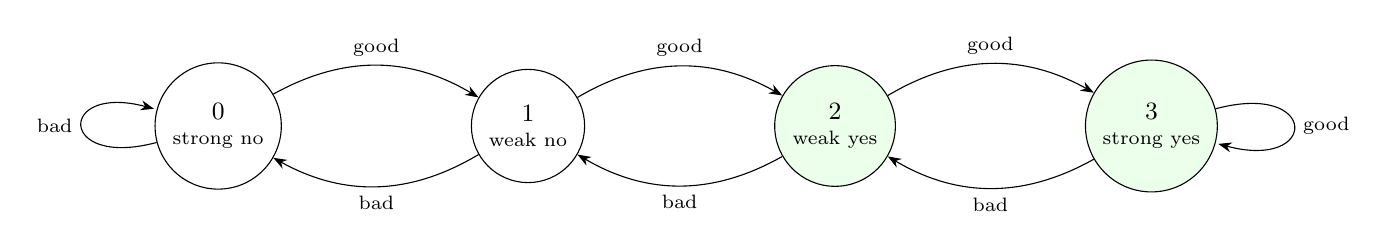
\begin{tikzpicture}[->,>=Stealth,node distance=24mm,auto,
  st/.style={circle,draw,minimum size=12mm,font=\small,align=center}]
  \node[st] (0) {0\\[-2pt]\scriptsize strong no};
  \node[st,right=of 0] (1) {1\\[-2pt]\scriptsize weak no};
  \node[st,right=of 1,fill=green!8] (2) {2\\[-2pt]\scriptsize weak yes};
  \node[st,right=of 2,fill=green!8] (3) {3\\[-2pt]\scriptsize strong yes};
  \path (0) edge[bend left] node{\scriptsize good} (1)
        (1) edge[bend left] node{\scriptsize good} (2)
        (2) edge[bend left] node{\scriptsize good} (3)
        (3) edge[bend left] node{\scriptsize bad} (2)
        (2) edge[bend left] node{\scriptsize bad} (1)
        (1) edge[bend left] node{\scriptsize bad} (0)
        (0) edge[loop left] node{\scriptsize bad} (0)
        (3) edge[loop right] node{\scriptsize good} (3);
\end{tikzpicture}
\end{center}
Start state: 1. A turn is \emph{good} when \f{advantage} $\ge 1 + \text{margin}$ \textbf{and} the history
allows it (next part).

\subsubsection*{Fight history}
\begin{lstlisting}[language=Rust]
pub struct History {
    pub results: u8,             // last 8 exchanges, newest in bit 0: 1 = we dealt >= we took
    pub len: u8,                 // how many are recorded (max 8)
    pub vs_kind: [Ctr2; 13],     // per enemy champion type: fights go well / badly
}
// history allows a fight unless: vs_kind[enemy] is "strong no", or the last 3 exchanges were all lost
let history_ok = !hist.bad_against(e.kind) && hist.recent_losses(3) < 3;
\end{lstlisting}
An \emph{exchange} is one turn near an enemy champion (within its range + 2): damage we dealt is the drop
in the watched enemy's health since our last turn; damage we took counts only when an enemy champion
could hit us. Turns with neither are not recorded.

\subsubsection*{Hysteresis gate (live: COMBAT\_FSM bit 64)}
The other layers still choose this turn's action; the gate only blocks a switch between fighting and fleeing
that the counter doesn't support. The memory is one value, \f{fsm\_fighting} $\in$ \{none, fighting,
fleeing\}, reset when no enemy is in view:
\begin{center}
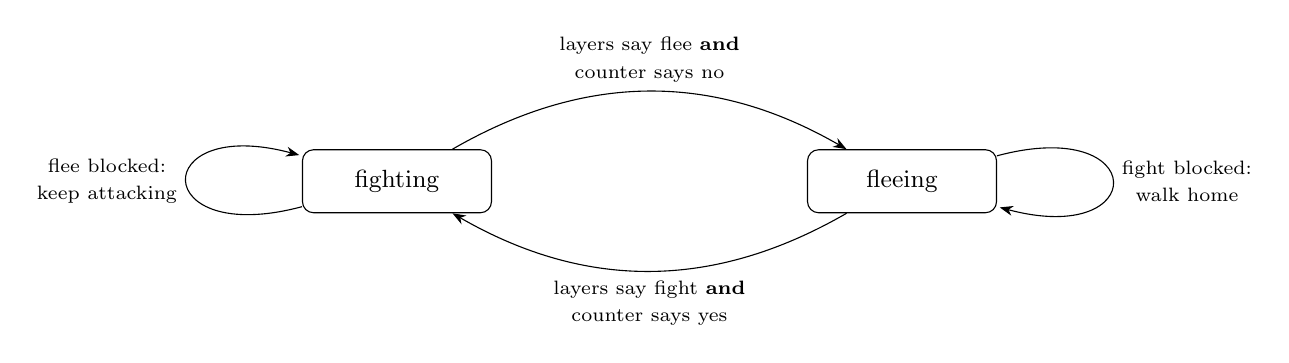
\begin{tikzpicture}[->,>=Stealth,node distance=40mm,auto,
  st/.style={rounded corners,draw,minimum width=24mm,minimum height=8mm,font=\small}]
  \node[st] (f) {fighting};
  \node[st,right=of f] (r) {fleeing};
  \path (f) edge[bend left] node[align=center]{\scriptsize layers say flee \textbf{and}\\[-2pt]\scriptsize counter says no} (r)
        (r) edge[bend left] node[align=center,below]{\scriptsize layers say fight \textbf{and}\\[-2pt]\scriptsize counter says yes} (f)
        (f) edge[loop left] node[align=center]{\scriptsize flee blocked:\\[-2pt]\scriptsize keep attacking} (f)
        (r) edge[loop right] node[align=center]{\scriptsize fight blocked:\\[-2pt]\scriptsize walk home} (r);
\end{tikzpicture}
\end{center}
\begin{lstlisting}[language=Rust]
let kept = match self.fsm_fighting {
    // was fighting, told to flee: only if the counter agrees (safety overrides always win)
    Some(true) if flees && self.fsm.fight.yes() && !matches!(mode, Mode::Override(_)) =>
        if ranged_vs_melee { Intent::Kite(e.pos) } else { Intent::Engage(e.pos) },
    // was fleeing, told to fight: only if the counter agrees
    Some(false) if fights && !self.fsm.fight.yes() => Intent::WalkHome,
    _ => intent,
};
\end{lstlisting}
\textbf{Points to criticise:} the counter is updated from the same advantage estimate the layers use, so it
filters noise but can't correct a wrong estimate; the gate never overrides the low-health safety rule.

\subsubsection*{Full combat state machine (COMBAT\_FSM bit 1 alone: off)}
Kept in \f{crates/bc-core/src/combat.rs} for future work; measured worse (\S\ref{sec:can}).
\begin{center}
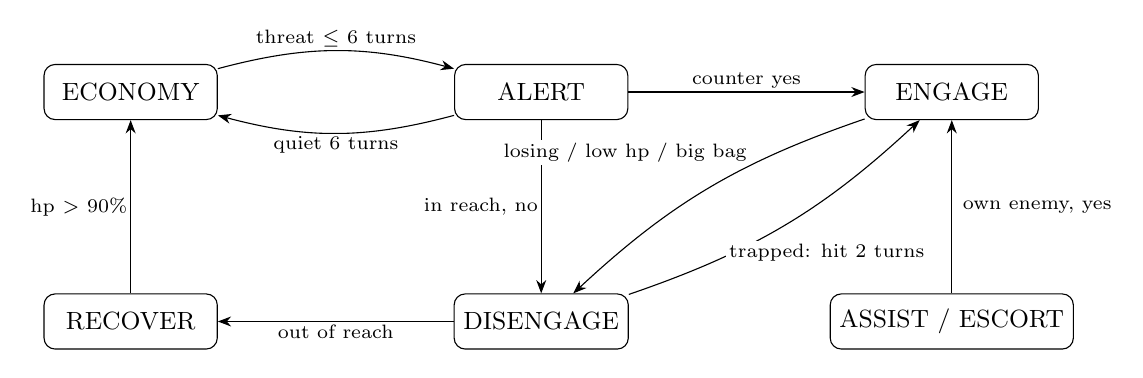
\begin{tikzpicture}[->,>=Stealth,node distance=22mm and 30mm,
  st/.style={rounded corners,draw,minimum width=22mm,minimum height=7mm,font=\small},
  lb/.style={font=\scriptsize,fill=white,inner sep=1pt}]
  \node[st] (e) {ECONOMY};
  \node[st,right=of e] (a) {ALERT};
  \node[st,right=of a] (g) {ENGAGE};
  \node[st,below=of e] (r) {RECOVER};
  \node[st,below=of a] (d) {DISENGAGE};
  \node[st,below=of g] (h) {ASSIST / ESCORT};
  \draw (e) to[bend left=15] node[lb,above]{threat $\le$ 6 turns} (a);
  \draw (a) to[bend left=15] node[lb,below]{quiet 6 turns} (e);
  \draw (a) -- node[lb,above]{counter yes} (g);
  \draw (a) -- node[lb,left]{in reach, no} (d);
  \draw (g) to[bend right=12] node[lb,pos=0.35,above left]{losing / low hp / big bag} (d);
  \draw (d) to[bend right=12] node[lb,pos=0.4,below right,xshift=-4mm]{trapped: hit 2 turns} (g);
  \draw (d) -- node[lb,below]{out of reach} (r);
  \draw (r) -- node[lb,left]{hp $>$ 90\%} (e);
  \draw (h) -- node[lb,right,xshift=1mm]{own enemy, yes} (g);
\end{tikzpicture}
\end{center}
States have minimum dwell times (ENGAGE 2 turns); ALERT blocks captures and deliveries when a threat can
arrive before the channel ends. Its cost was economic: champions spent too many turns not farming.

\subsection{Decision formulas}
\paragraph{Fight advantage} (\f{crates/bc-brain/src/router.rs}):
\begin{lstlisting}[language=Rust]
let our_dps   = (ctx.my_dps + ctx.ally_dps_near).max(1.0);         // live stats, items included
let their_dps = (e.dps * f32::from(ctx.enemies_in_range.max(1))).max(1.0);
let advantage = (ctx.hp / their_dps) / (e.hp / our_dps).max(0.1)  // time to kill us / time to kill them
              * ctx.fight_bias.exp();                               // learned FIGHT weights
// fight if advantage >= 1 + margin - bounty + risk
//   margin = fight_margin% x (255 - aggression) / 127;  bounty 0.2 if the enemy carries >= 20 gems
//   risk 1.0 if we carry a big bag;  enemy dps x (1 + 0.5 x missing hp) for Heart of Ruin
\end{lstlisting}
\paragraph{Camp choice} (\f{bots/main/src/bot.rs}, \f{choose\_target}), per camp group:
\[
\text{score} = \frac{\text{value}}{\text{dist}\cdot w_{\text{dist}} + \text{clear}\cdot w_{\text{clear}} + \max(0, \text{eta}-\text{dist}) + 5}
\times e^{\,\text{TARGET}\cdot\phi} \times (1.3\,w_{\text{hyst}} \text{ if current target})
\]
where
\begin{itemize}
\item value $= (\text{gems}\cdot w_{\text{gem}} + 0.6\,\text{gold}\cdot w_{\text{gold}}) \,/\, (1 + \text{max strength}/100 \cdot w_{\text{strength}})$;
\item clear $= \text{group HP} / \text{our live damage}$ (turns to kill it alone);
\item eta $=$ rounds until it respawns.
\end{itemize} The $w$ are the trained W dials. \emph{Missing today (being tested):} survival
($\text{kill time} > 3 \times \text{survival time} \Rightarrow \times 0.1$), the early ramp
($\div\, 1 + \max(0, \text{clear} - 20)/20$) and live camp HP.

\paragraph{Delivering gems} (\f{policy::should\_tribute}): deliver when the bag reaches TRIBUTE\_MAX, or
$\text{bag} \ge \text{TRIBUTE\_MIN} + \text{dist to altar} \times \text{scale}/10$, halved when hurt, threatened
or after round 1800; within 2 tiles of an altar the requirement is at most 5 gems.

\paragraph{Kill assist} (bit 2): if no enemy champion is within 4 tiles, we carry less than a big bag, our
health is over 40\%, and the shared sighting is at most 1 round old, within 4 tiles and at $\le$ 50\% health
(quarters 0--1) $\Rightarrow$ engage it.

\paragraph{Help on my way} (bit 128): the goal is where the current intent leads (camp centre, nearest altar
or home); we answer the 1-bit help flag only if $\text{dist}(me, p) \le 10$ and
$\text{dist}(me,p) + \text{dist}(p, goal) - \text{dist}(me, goal) \le 4$ (Chebyshev distances).

\subsection{League daemon logic}\label{sec:pressure}
\begin{lstlisting}[language=Python]
def cycle():                          # harness/league.py, one round
    integrate()                       # git fetch + rebase; champion.json is merged per map
    seed_maps(); apply_champion()     # every pool map has a theta; pack.bin follows champion.json
    maybe_release()                   # lead + --auto-submit: upload if due (also at the end)
    if lead: watch(); refresh_maps(); sync()   # ladder games, map pool, top-10 mimics
    if every 3rd round and no map still needs bootstrap: evolve_mimic()
    else: train()                     # 8 antithetic ES copies of one map's theta vs 5 opponents
    publish(champion.json, pack.bin)  # on a promotion or every 30 min (try counts)
    maybe_release()

def release_decision(ch, led, now):   # upload v if all hold
    newer = ch["version"] > live_version
    gap   = now - last_upload_time >= 3 * 3600
    why   = any loss since the last upload  or  bench(v) >= bench(live) + 0.05

def map_pressure(led, now):           # used when no open loss of the live version is queued
    for loss in led["losses"] (except needs-human):
        w = exp(-(now - loss.time) / 24h) * (2 if the live version lost it else 1)
        pressure[loss.map] += w
# pick map ~ (pressure[m] + 0.1 * max pressure + 0.05) * (1.1 - local win rate on m)
\end{lstlisting}
\paragraph{Promotion gate:} a copy replaces the champion's $\theta$ on that map only if its fitness
(win $+ 0.25\,$gem lead $- 0.01\,$deaths) beats the champion by 0.04 on the same games, it wins the
head-to-head ($\ge$ 0.5), it is at least as good on 3 fresh opponents, and it runs out of fuel at most
twice as often. \paragraph{Merging two PCs:} \f{merge\_champion} is a 3-way merge per map; if both sides
changed the same map, a head-to-head on that map decides; promotion history is unioned and renumbered.

\end{document}
